\documentclass[10pt,a4paper]{report}
\usepackage[utf8]{inputenc}
\usepackage[english]{babel}
\usepackage[T1]{fontenc}
\usepackage{amsmath}
\usepackage{amsfonts}
\usepackage{graphicx}
\usepackage{lmodern}
\usepackage{amssymb}
\usepackage{verbatim}
\usepackage{float}
\usepackage{amsthm}
\usepackage{hyperref}
\title{\LARGE{Algorithms for Computational Logic} \\ \vspace{0.5cm} \normalsize{Summary}}
\date{}

\begin{document}
\maketitle
\tableofcontents

\chapter{SAT and Modeling with SAT}
\section{Cardinality Constraints}
In order to handle cardinality constraints we have two options: encode the cardinality constraints to CNF and use a SAT solver, or use a pseudo boolean (PB) solver.
\subsection{AtMost1}
\begin{itemize}
\item $\sum_{j=1}^n x_j = 1$ can be encoded with $\left(\sum_{j=1}^n x_j \leq 1\right) \land \left(\sum_{j=1}^n x_j \geq 1\right)$
\item $\sum_{j=1}^n x_j \geq 1$ can be encoded with $(x_1 \lor x_2 \lor ... \lor x_n)$
\item $\sum_{j=1}^n x_j \leq 1$ can be encoded with:
\begin{itemize}
\item Pairwise encoding
\item Sequential counter encoding
\item Bitwise encoding
\end{itemize}
\end{itemize}
\subsubsection{Sequential Counter}
In order to realize this encoding, we need to add new variables $s_i$ for the fact "there is a 1 on some position $1..i$":
$$
s_i \text{ is true if } \sum_{j=1}^i x_j \geq 1
$$
Encoding $\sum_{j=1}^n x_j \leq 1$ with sequential counter:
\begin{align*}
&(\neg x_1 \lor s_1) \land\\
&(\neg x_i \lor s_i), i \in 2..n-1 \land\\
&(\neg s_{i-1} \lor s_i), i \in 2..n-1 \land\\
&(\neg x_i \lor \neg s_{i-1}), i \in 2..n
\end{align*}
If $x_j = 1$, then all $s_i$ variables are assigned and all other $x$ variables must take value 0. There are $\mathcal{O}(n)$ clauses and $\mathcal{O}(n)$ auxiliary variables.
\subsubsection{Bitwise Encoding}
In bitwise encoding, we represent the constraint $\sum_{j=1}^n x_j \leq 1$ by encoding the index of the potential true variable in binary. For this, we add new auxiliary variables:
$$
v_0, ... v_r-1;\; r=\lceil \log n \rceil (\text{with } n > 1)
$$
Each variable $x_j$ is assigned a unique binary number that represents its index. Then, for each variable $x_j$ with binary index representation $i$, we create clauses that enforce the condition: 
\begin{itemize}
    \item If $x_j = 1$, assignment to $v_i$ variables must encode $j - 1$, and all other $x$ variables must take value 0
    \item If all $x_j = 0$, any assignment to $v_i$ variables is consistent
\end{itemize}
For example, $x_1 + x_2 + x_3 \leq 1$:\\
\begin{minipage}{0.4\textwidth} 
    \centering
    \begin{table}[H]
        \begin{tabular}{ccc}
              & $j-1$ & $v_1v_0$ \\ \cline{1-3}
        $x_1$ & 0     & 00   \\
        $x_2$ & 1     & 01  \\
        $x_3$ & 2     & 10   
        \end{tabular}
    \end{table}
\end{minipage}
\begin{minipage}{0.55\textwidth} 
    \begin{align*}
        &(\neg x_1 \lor \neg v_1) \land (\neg x_1 \lor \neg v_0)\\
        &(\neg x_2 \lor \neg v_1) \land (\neg x_2 \lor v_0)\\
        &(\neg x_3 \lor v_1) \land (\neg x_3 \lor \neg v_0)\\
    \end{align*}
\end{minipage}
There are $\mathcal{O}(n\log n)$ clauses and $\mathcal{O}(\log n)$ auxiliary variables

\subsection{General Cardinality Constraints}
Constraints of the form $\sum_{j=1}^n x_j \leq k$ or $\sum_{j=1}^n x_j \geq k$ can be added with:
\begin{itemize}
    \item Sequential Counters
    \item BDDs
    \item Sorting Networks
    \item Cardinality Networks
    \item Totalizer
\end{itemize}
\subsubsection{Sequential Counter Encoding}
For each variable $x_i$, create k additional variables $s_{i,j}$ that are used as counters:
\begin{itemize}
    \item $s_{i,j} = 1$ if at least $j$ variables $\{x_1 ... x_i\}$ are assigned value 1
    \item $s_{i,j} = 0$ if at most $j - 1$ variables $\{x_1 ... x_i\}$ are assigned value 1
\end{itemize}
Encoding:
\begin{figure}[H]
    \centering
    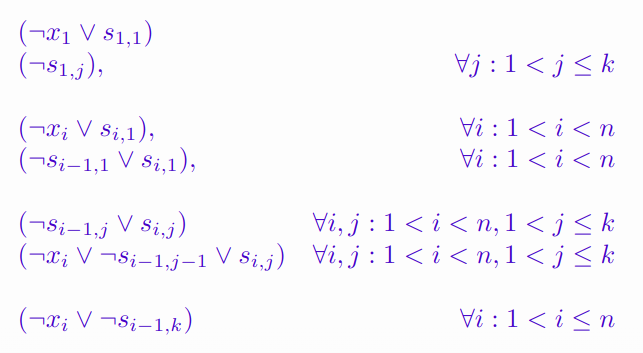
\includegraphics[scale=0.4]{1.png}
\end{figure}
\subsubsection{Totalizer Encoding}
In this encoding we count in unary how many of the $n$ variables $(x_1 ... x_n)$ are assigned to 1. It can be visualized as a tree:
\begin{itemize}
    \item Each node is ($name$ : $variable$ : $sum$)
    \item Root node has the output variables $(o_1 ... o_n)$ that count how many variables are assigned to 1
    \item Literals are at the leaves
    \item Each node counts in unary how many leaves are assigned to 1 in its subtree
    \item Example: if $b_2 = 1$, then at least 2 of the leaves $(x_3, x_4, x_5)$ are
    assigned to 1
\end{itemize}
\begin{figure}[H]
    \centering
    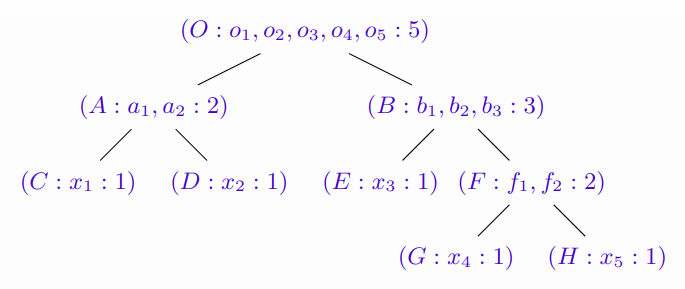
\includegraphics[scale=0.5]{2.png}
\end{figure}
To encode $x_1 + x_2 + x_3 + x_4 + x_5 \leq 3$ just set $o_4=0$ and $o_5=0$.\\
Encoding:
\begin{figure}[H]
    \centering
    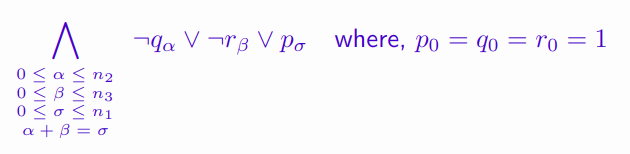
\includegraphics[scale=0.5]{3.png}
\end{figure}
There are $\mathcal{O}(n\log n)$ new variables and $\mathcal{O}(n^2)$ new clauses

\section{SAT Algorithms}
\subsection{DPLL Solvers}
\begin{figure}[H]
    \centering
    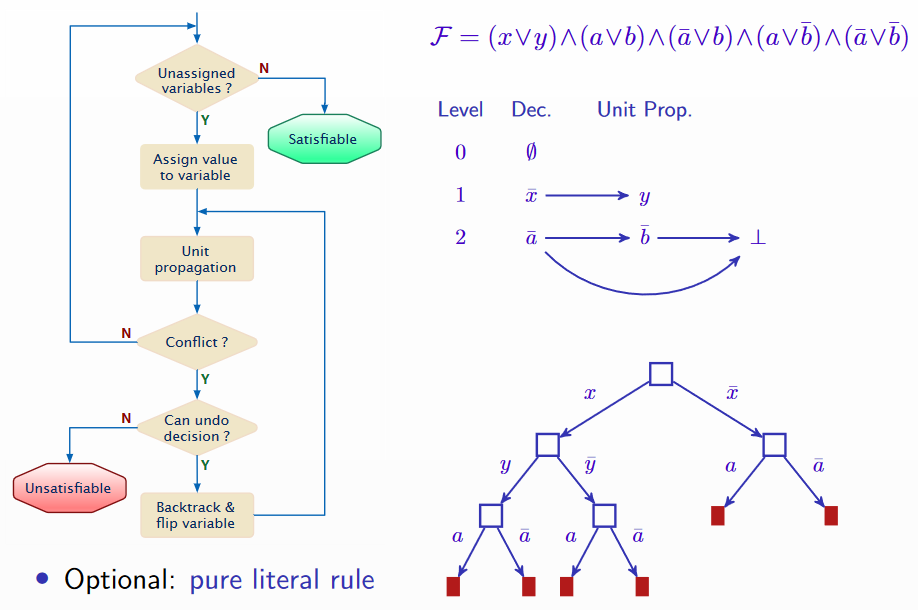
\includegraphics[scale=0.5]{4.png}
\end{figure}
\subsection{CDCL Solvers}
CDCL solvers extend DPLL solvers with clause learning and non-chronological backtracking, search restarts, lazy data structures, conflict-guided branching, etc.
\subsubsection{Clause Learning}
\begin{figure}[H]
    \centering
    
\includegraphics[scale=0.5]{5.png}
\end{figure}
And after backtracking:
\begin{figure}[H]
    \centering
    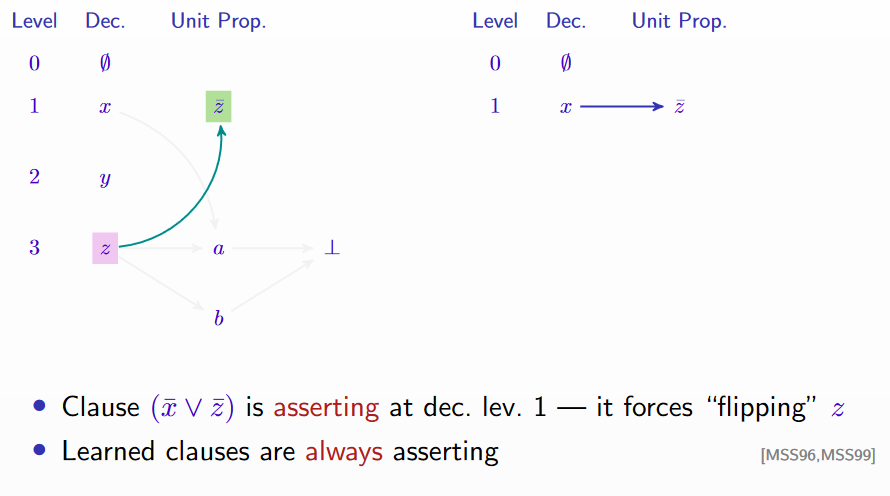
\includegraphics[scale=0.5]{6.png}
\end{figure}
\subsubsection{Unique Implication Points}
\begin{figure}[H]
    \centering
    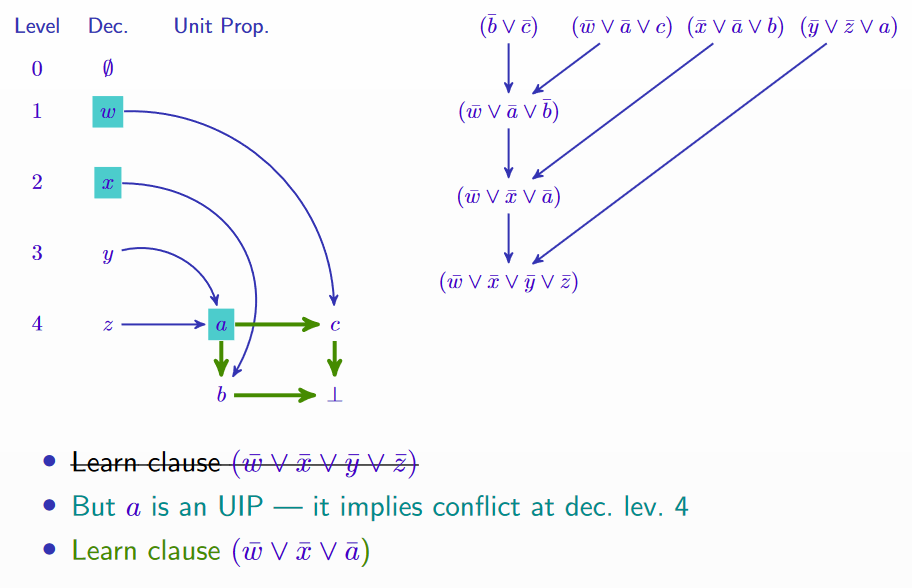
\includegraphics[scale=0.5]{7.png}
\end{figure}
\subsubsection{Clause Minimization}
\begin{figure}[H]
    \centering
    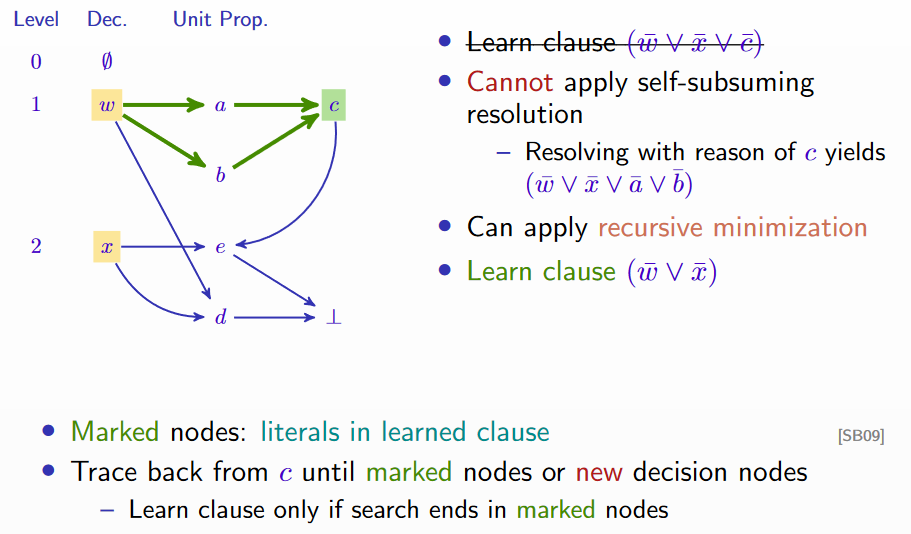
\includegraphics[scale=0.5]{8.png}
\end{figure}

\chapter{Optimization problems and SAT-Based Problem Solving}
A set of constraints is overconstrained if it is inconsistent. In a given an unsatisfiable formula, there may be several explanations for its unsatisfiability. The goal of MaxSAT is to find largest subset of clauses that is satisfiable.
\begin{figure}[H]
    \centering
    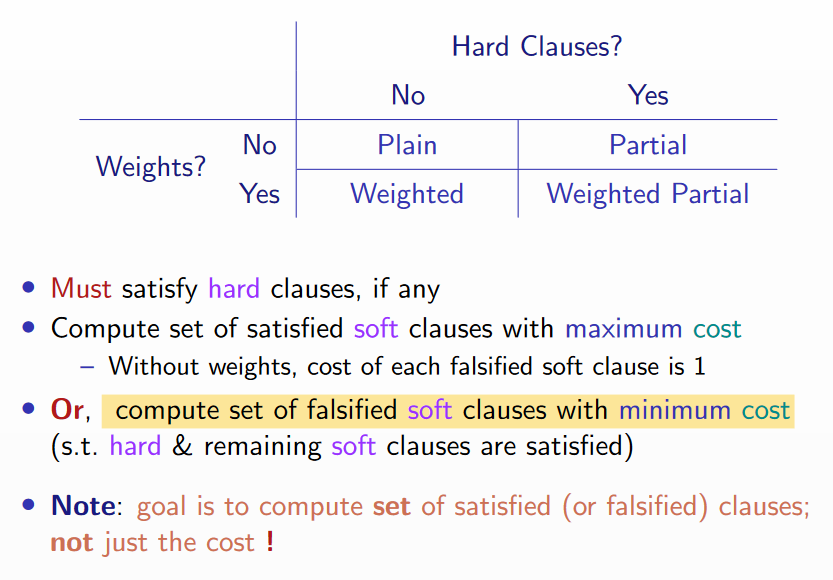
\includegraphics[scale=0.5]{9.png}
\end{figure}

\section{MaxSAT Algorithms}
\subsection{Fu and Malik}
\begin{figure}[H]
    \centering
    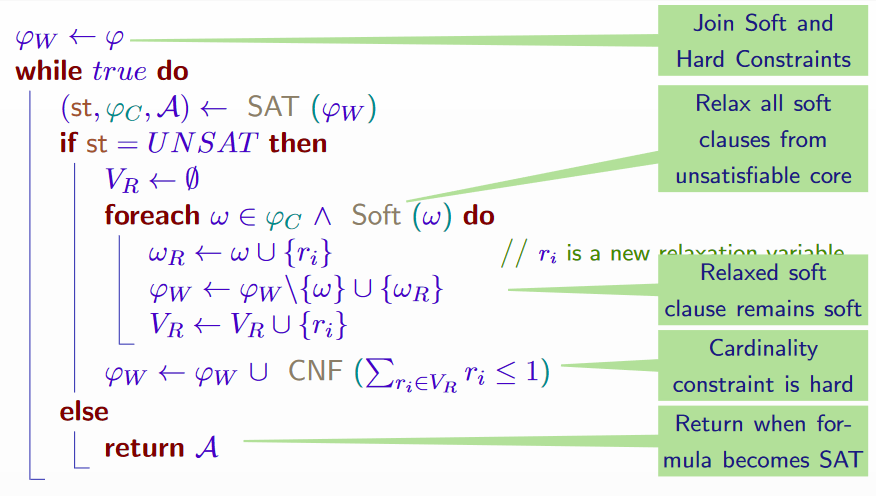
\includegraphics[scale=0.5]{10.png}
\end{figure}
\subsection{MSU3}
\begin{figure}[H]
    \centering
    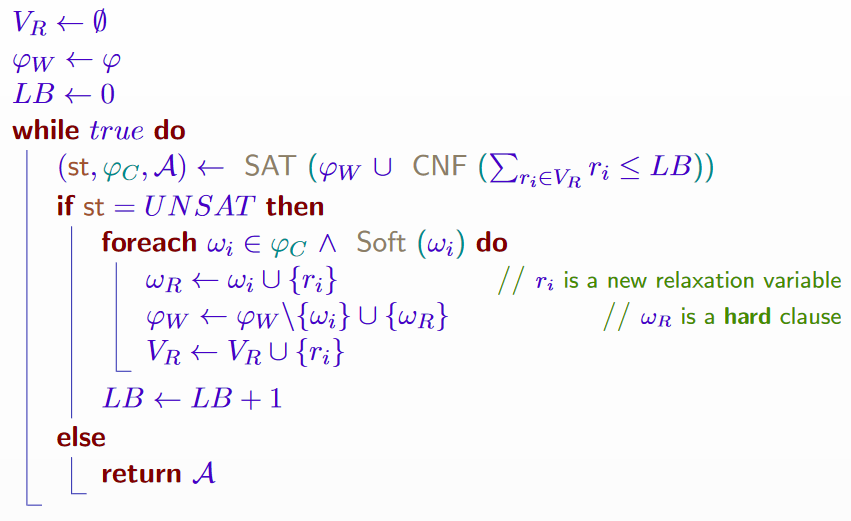
\includegraphics[scale=0.5]{11.png}
\end{figure}

\section{Minimal Unsatisfiable Subsets}
Given $\mathcal{F}$ unsatisfiable, $\mathcal{M} \subseteq \mathcal{F}$ is a MUS iff $\mathcal{M}$ is unsatisfiable and $\forall_{c \in \mathcal{M}}, \mathcal{M} \setminus \{c\}$ is satisfiable.
\subsection{Algorithms}
The following algorithms may be used to identify minimal unsatisfiable subsets.
\subsubsection{Deletion-Based}
\begin{figure}[H]
    \centering
    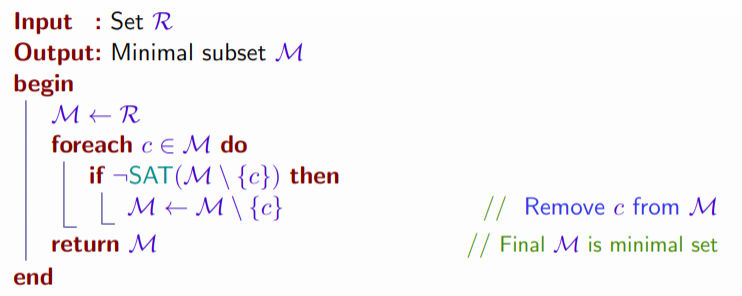
\includegraphics[scale=0.5]{12.png}
\end{figure}
\subsubsection{Insertion-Based}
\begin{figure}[H]
    \centering
    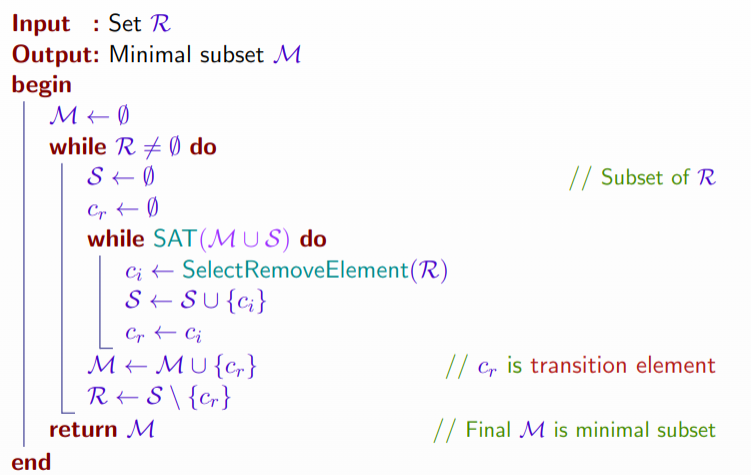
\includegraphics[scale=0.5]{13.png}
\end{figure}
\subsubsection{Dichotomic}
\begin{figure}[H]
    \centering
    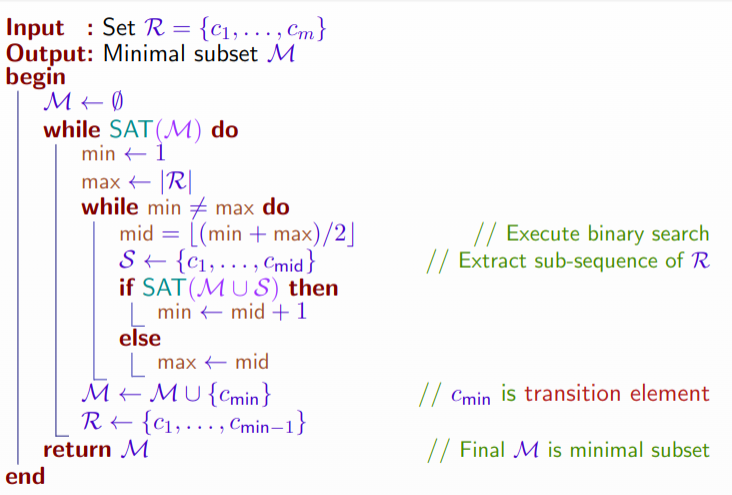
\includegraphics[scale=0.5]{14.png}
\end{figure}

\section{Minimal Correction Subsets}
$\mathcal{C} \subseteq \mathcal{F}$ is an MCS iff $\mathcal{F} \setminus \mathcal{C}$ is satisfiable and $\forall_{c \in \mathcal{C}}, \mathcal{F} \setminus (\mathcal{C} \setminus \{c\})$ is unsatisfiable.
\subsection{Algorithms}
The following algorithms may be used to identify minimal correction subsets.
\subsubsection{Basic Linear Search}
\begin{itemize}
    \item Let $\mathcal{S} \subseteq \mathcal{F}$, such that $\mathcal{S}\nvDash \bot$, initially $\mathcal{S} = \emptyset$
    \item Let $\mathcal{C} \subseteq \mathcal{F}$, such that $\forall_{c \in \mathcal{C}}, \mathcal{S} \cup \{c\} \vDash \bot $, initially $\mathcal{C} = \emptyset$
    \item At each iteration, analyze one clause of $c \in \mathcal{F} \setminus (\mathcal{S} \cup \mathcal{C})$:
    \begin{itemize}
        \item If $\mathcal{S} \cup \{c\} \vDash \bot$, then add $c$ to $\mathcal{C}$, i.e. $c$ is part of MCS
        \item If $\mathcal{S} \cup \{c\} \nvDash \bot$, then add $c$ to $\mathcal{C}$, i.e. $c$ is part of MCS
    \end{itemize}
\end{itemize}
There are $\mathcal{O}(m)$ calls to the oracle. An example:
\begin{figure}[H]
    \centering
    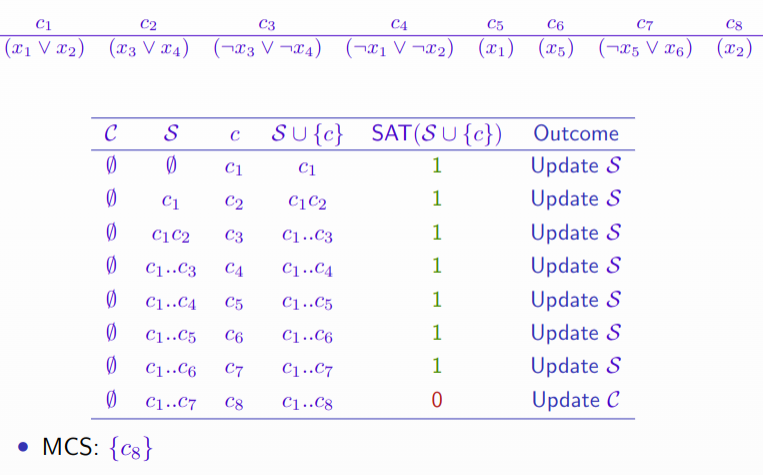
\includegraphics[scale=0.4]{15.png}
\end{figure}
\subsubsection{Clause D}
\begin{itemize}
    \item Pick an assignment and let $\mathcal{S} \subseteq \mathcal{F}$ be the satisfied clauses and $\mathcal{U} \subseteq \mathcal{F}$ be the falsified clauses, with $\mathcal{F} = \mathcal{S} \cup \mathcal{U}$
    \item Repeat:
    \begin{itemize}
        \item Create clause $D = \cup_{l \in c, c \in \mathcal{U}} l$
        \item If $\mathcal{S} \cup \{D\} \vDash \bot$, then $\mathcal{U}$ is MCS: Report MCS and terminate
        \item If $\mathcal{S} \cup \{D\} \nvDash \bot$, then add to $\mathcal{S}$ the satisfied clauses in $\mathcal{U}$, remove from $\mathcal{U}$ the satisfied clauses and loop
    \end{itemize}
\end{itemize}
There are $\mathcal{O}(m-r)$ calls to the oracle, where $r$ is the size of the smallest MCS. An example:
\begin{figure}[H]
    \centering
    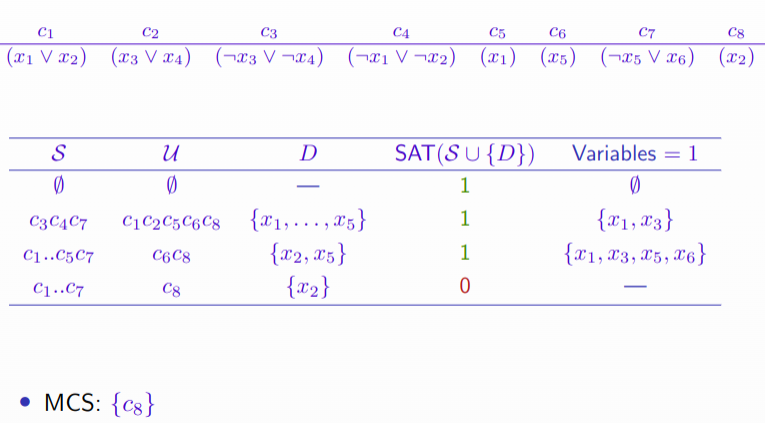
\includegraphics[scale=0.4]{16.png}
\end{figure}


\chapter{Satisfiability Modulo Theories}
\chapter{Answer Set Programming}
\end{document}
